% !TeX TS-program = xelatex
% !BIB TS-program = bibtex

% Full instructions available at:
% https://github.com/elauksap/focus-beamertheme

\documentclass{beamer}
\usetheme{focus}
\usepackage{booktabs}

\title{Data vs. Model Centric ML Fairness Testing}
\subtitle{An Empirical Study}
\author{Arumoy Shome\texorpdfstring{\\}{,} Lu{\'\i}s
  Cruz\texorpdfstring{\\}Arie van Deursen}
\institute{Delft University of Technology}
\date{\today}

% Footline info is printed only if [numbering=fullbar].
%\footlineinfo{Custom footline text}

\begin{document}
\begin{frame}
  \maketitle
\end{frame}

% Use starred version (e.g. \section*{Section name})
% to disable (sub)section page.
\section{Introduction}
\begin{frame}{Research Questions}
  \begin{itemize}
  \item{\textbf{RQ1.}} \textbf{What is the relationship between DFM
    and MFM as the underlying data distribution chages?}
  \item{\textbf{RQ2.}} \textbf{What is the relationship between DFM and
    MFM across various training sample sizes?}
  \item{\textbf{RQ3.}} \textbf{What is the relationship between DFM and
    MFM across various feature sample sizes?}
  \end{itemize}
\end{frame}

\section{Background and Related Work}
%% TODO
\section{Experimental Design}
\setbeamertemplate{caption}[numbered]
\begin{frame}[t]{Datasets, ML Models and Fairness Metrics}
  \begin{table}
    \centering
    \caption{Datasets used in the study}
    \begin{tabular}{llr}
      \toprule
      \textbf{Name} & \textbf{Prot.} & \textbf{Total Examples}\\
      \midrule
      German Credit \cite{CITEME} & age, sex & 1000\\
      Compas Score \cite{CITEME} & race, sex & 6167\\
      Medical Survey 2021 \cite{CITEME} & race & 15675\\
      Bank Marketing \cite{CITEME} & age & 30488\\
      Adult Income \cite{CITEME} & race, sex & 45222\\
      \bottomrule
    \end{tabular}
    \label{tab:datasets}
  \end{table}
\end{frame}

\begin{frame}[t]{Group Fairness Metrics}
\begin{equation}
  DI_{data} = \frac{P(Y=1|D=0)}{P(Y=1|D=1)}
  \label{eq:di-data}
\end{equation}

\begin{equation}
  DI_{model} = \frac{P(\hat{Y}=1|D=0)}{P(\hat{Y}=1|D=1)}
  \label{eq:di-model}
\end{equation}

\begin{equation}
  SPD_{data} = P(Y=1|D=0)-P(Y=1|D=1)
  \label{eq:spd-data}
\end{equation}

\begin{equation}
  DI_{model} = P(\hat{Y}=1|D=0)-P(\hat{Y}=1|D=1)
  \label{eq:spd-model}
\end{equation}
\end{frame}

\begin{frame}[c]{Fairness evaluation}
  \begin{figure}[c]
  \centering
  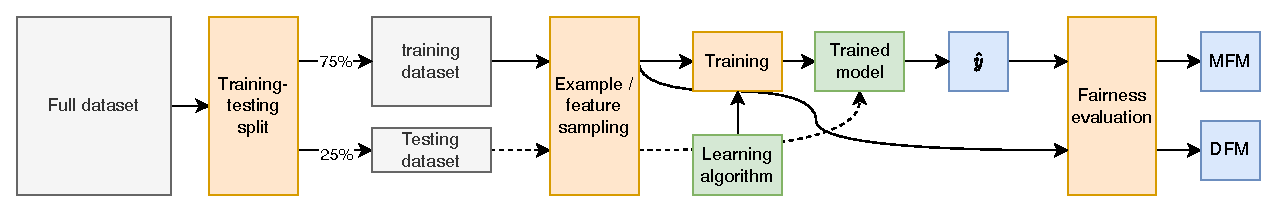
\includegraphics[width=0.95\linewidth]{method.pdf}
  \caption{Methodology for data collection and analysis}
  \label{fig:method}
\end{figure}

  
\end{frame}
\section{Results}
\begin{frame}{Overview of Results}
  \begin{columns}[t]
    \column{0.45\textwidth}
    \begin{center}
      \textbf{Full training set experiments}
    \end{center}
    \begin{enumerate}
    \item What is the relationship between DFM and MFM?
    \item What is the relationship between DFM and MFM as the
      underlying data distribution changes?
    \item How does the training sample size affect the relationship
      between DFM and MFM?
    \end{enumerate}
    \column{0.45\textwidth}
    \begin{center}
      \textbf{Training and feature sample size experiments}
    \end{center}
    \begin{enumerate}
    \item What is the relationship between DFM and MFM across training
      sample sizes?
    \item What is the relationship between DFM and MFM across
      feature sample sizes?
    \end{enumerate}
  \end{columns}
\end{frame}

\subsection{Full training set experiments}
\begin{frame}{What is the relationship between DFM and MFM?}
  
\end{frame}

\begin{frame}{What is the relationship between DFM and MFM as the
    underlying data distribution changes?}
  
\end{frame}

\begin{frame}{How does the training sample size affect the
    relationship between DFM and MFM?}
  
\end{frame}
\begin{frame}[focus]
  Thanks for using \textbf{Focus}!
\end{frame}

\appendix
\begin{frame}{References}
  \nocite{*}
  \bibliography{report}
  \bibliographystyle{named}
\end{frame}
\end{document}
